\documentclass[tikz]{standalone}
\usepackage{pgfplots}
\pgfplotsset{compat=1.18}
\begin{document}
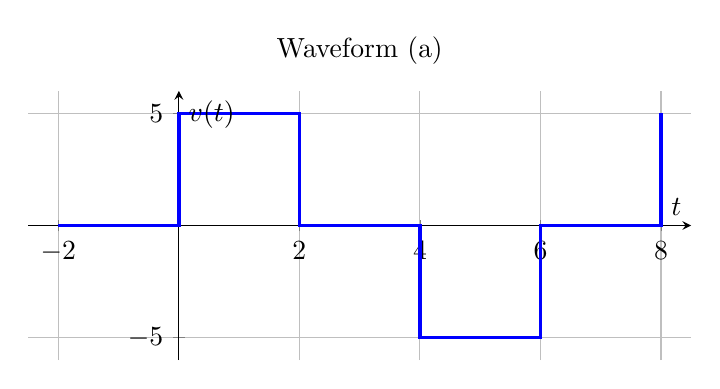
\begin{tikzpicture}
\begin{axis}[
    axis lines = middle,
    xlabel = {$t$},
    ylabel = {$v(t)$},
    xmin = -2.5, xmax = 8.5,
    ymin = -6, ymax = 6,
    xtick = {-2, 0, 2, 4, 6, 8},
    ytick = {-5, 0, 5},
    grid = both,
    width=10cm, height=5cm,
    title = {Waveform (a)}
]
\addplot[blue, very thick, no marks] coordinates {
    (-2, 0) (0, 0)
    (0, 5) (2, 5)
    (2, 0) (4, 0)
    (4, -5) (6, -5)
    (6, 0) (8, 0)
    (8, 5) % Start of next period
};
\end{axis}
\end{tikzpicture}
\end{document}
